\chapter{Implementação do Sistema desenvolvido} \label{cap:cap5}

Um fluxograma descrevendo as interações entre o usuário e ambiente virtual de treinamento que contempla todas as funcionalidades pode ser visto na 
Figura~\ref{fig:fluxogramaAmbiente}.

\begin{figure}[ht!]
    \centering
    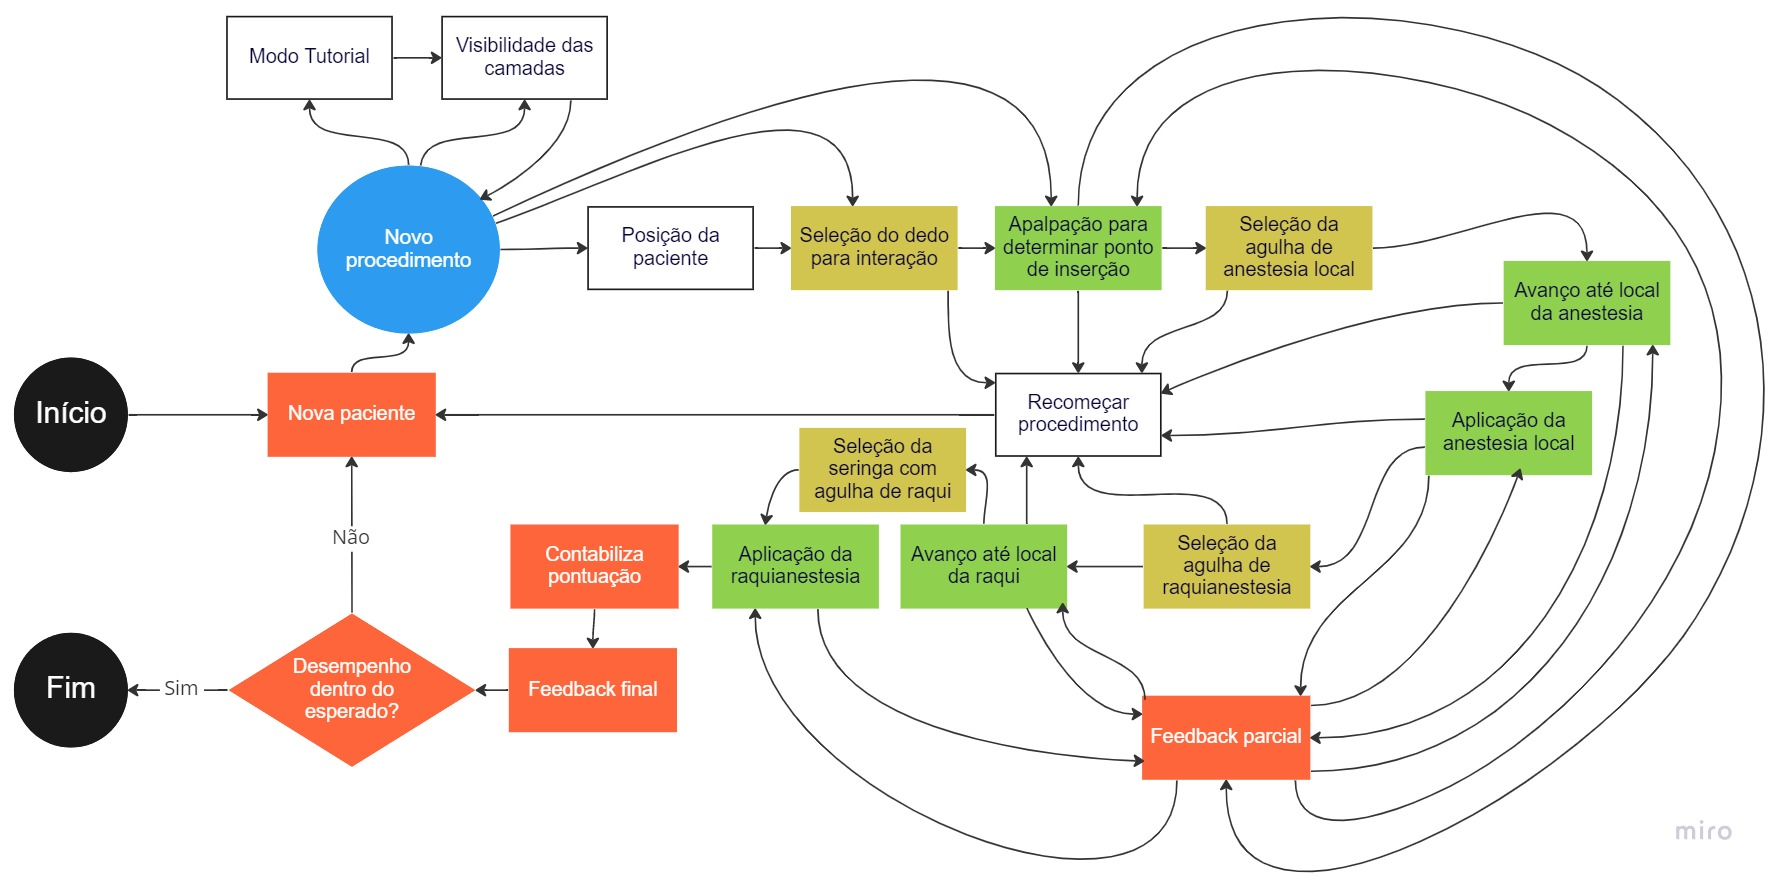
\includegraphics[width=0.98\linewidth]{capitulos/figuras/fluxograma-ambiente-desenvolvido.jpg} 
    \caption{Fluxograma descrevendo tudo o que envolve a execução de cada novo procedimento no ambiente desenvolvido. Em branco estão as funcionalidades opcionais, em amarelo as interações que são feitas através de botões do háptico ou do teclado, em verde as interações que possuem retorno de forças do háptico e em vermelho as avaliações e retornos dados pelo sistema ao usuário.}
    \label{fig:fluxogramaAmbiente}
\end{figure}

Ao ser iniciado o sistema apresenta ao usuário uma paciente dentre as seis pré-configuradas ilustradas na Figura~\ref{fig:pacientesMaiorParaMenorIMCVisaoTroncoELateral}. Nesta figura existem pacientes com peso considerado normal, excesso de peso e obesas \cite{MTILLC2019}. O usuário deve, então, usar o dispositivo háptico para interagir com o ambiente virtual. Ao ser iniciado o sistema e a cada inicio de procedimento em uma nova paciente, ao movimentar o dispositivo háptico, o item que representa o dedo é movimentado no ambiente virtual de treinamento. O item no ambiente 3D que representa o dedo pode ser observado na Figura~\ref{fig:elementosDeInteracao} (a) do lado direito do tronco da paciente. Outro item a ser observado nesta imagem é uma esfera azul que indica onde foi o último toque do dedo no corpo da paciente. O último ponto tocado foi a estratégia definida para determinação da escolha do ponto de inserção da agulha na simulação. Nas Figuras~\ref{fig:elementosDeInteracao} (b) e (c) estão atrás do tronco da paciente, respectivamente, a seringa para anestesia local e a agulha usada para aplicação da raquianestesia. No momento da aplicação da raquianestesia, uma seringa é conectada no final da agulha como pode ser visto pela visão lateral na Figura~\ref{fig:agulhaRaquiSeringa}.

\begin{figure}[ht!]
    \centering
        \begin{tabular}{ccc}
        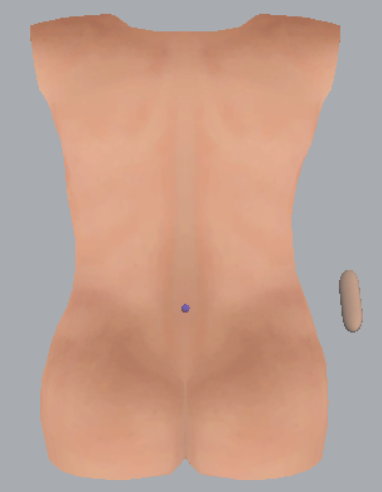
\includegraphics[width=0.3\linewidth]{capitulos/figuras/corpo-paciente-apos-apalpacao-dedo.png} & 
        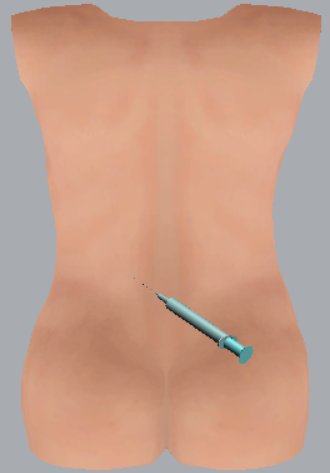
\includegraphics[width=0.27\linewidth]{capitulos/figuras/corpo-paciente-seringa.png} & 
        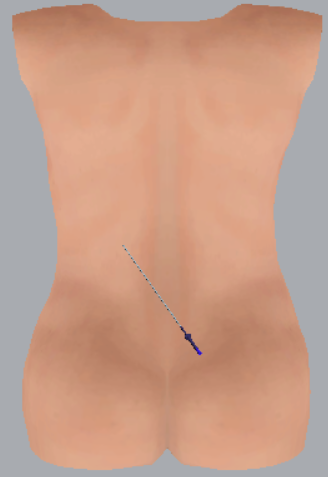
\includegraphics[width=0.27\linewidth]{capitulos/figuras/corpo-paciente-agulha-raqui.png} 
        \\
        (a) & (b) & (c)
        \end{tabular}
    \caption{Elementos 3D de interação com o ambiente representativos do: (a) Dedo (b) Seringa para anestesia local (c) Agulha de raquianestesia.}
    \label{fig:elementosDeInteracao}
\end{figure}

\begin{figure}[ht!]
    \centering
    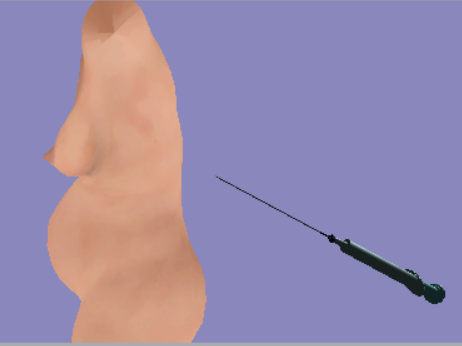
\includegraphics[width=0.4\linewidth]{capitulos/figuras/corpo-visao-lateral-agulhaRaquiSeringa.png} 
    \caption{Visão lateral do corpo da paciente com aproximação da agulha de raquianestesia com a seringa conectada.}
    \label{fig:agulhaRaquiSeringa}
\end{figure}

Cada procedimento no simulador é considerado como sendo finalizado no momento que é aplicada a raquianestesia, ou seja, ao ser pressionado o êmbolo da seringa conectada na agulha, desde que esta esteja dentro do corpo da paciente.
É necessário completar a execução de ao menos três procedimentos tendo a média das notas acima de seis para que a habilidade do usuário seja considerada como satisfatória. A nota final corresponde a média da nota obtida em todos os procedimentos executados. No casos de não se atingir a média seis nos três primeiros procedimentos será necessário executar tantos procedimentos quantos forem necessários para se chegar a média seis, considerando todos os procedimentos executados. Estas características foram inseridas no ambiente de treinamento e buscam aumentar a sua efetividade por meio do que é conhecido como a individualização em \textit{serious games} \cite{Sajjadi2022}.

A Tabela~\ref{tab:PontosNotaProcedimento} ilustra a pontuação para formação da nota de cada procedimento. Como nesta etapa de desenvolvimento do simulador estávamos sem contato direto com um anestesista para auxílio na determinação destas pontuações, foi feita uma proposta de pontuação inicial baseada no conhecimento obtido a partir dos estudos do procedimento, suas falhas e consequências. Para cada procedimento a nota inicia em zero. Itens feitos corretamente e na sequência correta tem pontuação positiva e itens feitos de forma incorreta ou não feitos tem pontuação negativa. Para algumas ações não feitas, ao invés da pontuação negativa, não é aplicada nenhuma penalização uma vez que a não execução correta já acarreta em penalização por não adicionar pontuação positiva na nota. O item que tem mais influência na pontuação é a aplicação na raquianestesia no local correto uma vez que isto é o que determina se a pessoa estará ou não corretamente anestesiada ao final do procedimento.

\begin{table}[!ht]
\begin{center}
\caption{Pontos para formarem a nota final de cada procedimento.}
\label{tab:PontosNotaProcedimento}
\begin{tabular}{|p{0.8\linewidth}|p{0.1\linewidth}|}
\hline
\textbf{Item executado} & \textbf{Ponto}\\
\hline\hline
Execução da apalpação para determinação do local de inserção da agulha & +1\\
%Perfuração do corpo com seringa ou agulha antes da apalpação & -1\\
Perfuração do corpo com seringa ou agulha antes da apalpação & -1\\
Anestesia local não aplicada & -1\\
Anestesia local aplicada com a seringa no local correto & +3\\
Avanço com a seringa até camadas indevidas (ex. ossos, espaço epidural) & -1\\
Perfuração do corpo da paciente duas ou três vezes (com seringa ou agulha) & -1\\
Perfuração do corpo da paciente quatro vezes ou mais (com seringa ou agulha) & -2\\
Inseriu a agulha de raquianestesia sem antes aplicar a anestesia local & -1\\
Aplicação da raquianestesia em local diferente do espaço subaracnóide & -3\\
Aplicação da raquianestesia no espaço subaracnóide & +6\\
\hline
\end{tabular}
\end{center}
\end{table}

São apresentados \textit{feedbacks} para o usuário durante e ao final dos procedimentos executados em cada uma das pacientes. As Figuras \ref{fig:sistemaExecucao1RaquiLocalIncorreto}, \ref{fig:sistemaExecucao2seringaCorreto}, \ref{fig:sistemaExecucao3faltouApalpacaoAnestesiaLocalIncorreto}, \ref{fig:sistemaExecucao4correto} e \ref{fig:sistemaExecucao5semApalpacaoCorreto} mostram uma sequência de possíveis execuções de anestesias, ilustrando diferentes erros e acertos durante cada procedimento que são visualizados no \textit{feedback} a direita durante a execução dos procedimentos e na janela de \textit{popup} ao final destes. 

\begin{figure}[ht!]
    \centering
    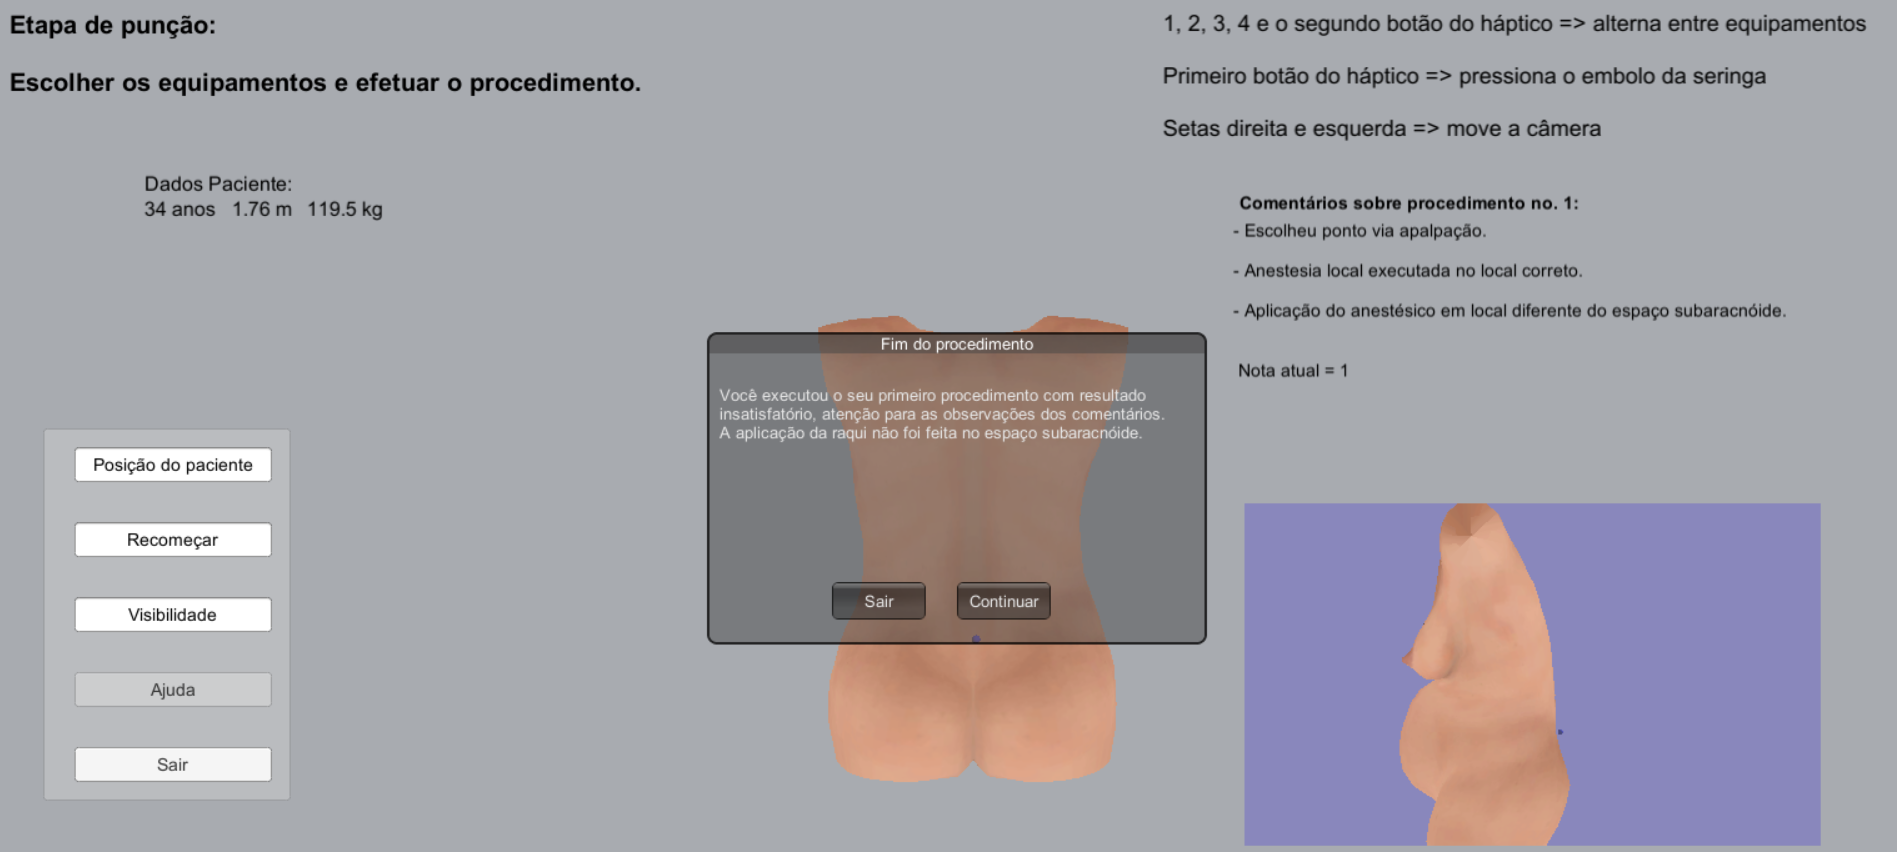
\includegraphics[width=\textwidth]{capitulos/figuras/sistema-exemplo-execucao-procedimento-1.png} 
    \caption{Ilustração de \textit{feedback} do ambiente após finalização de um primeiro procedimento onde a raquianestesia foi aplicada em local incorreto.}
    \label{fig:sistemaExecucao1RaquiLocalIncorreto}
\end{figure}

\begin{figure}[ht!]
    \centering
    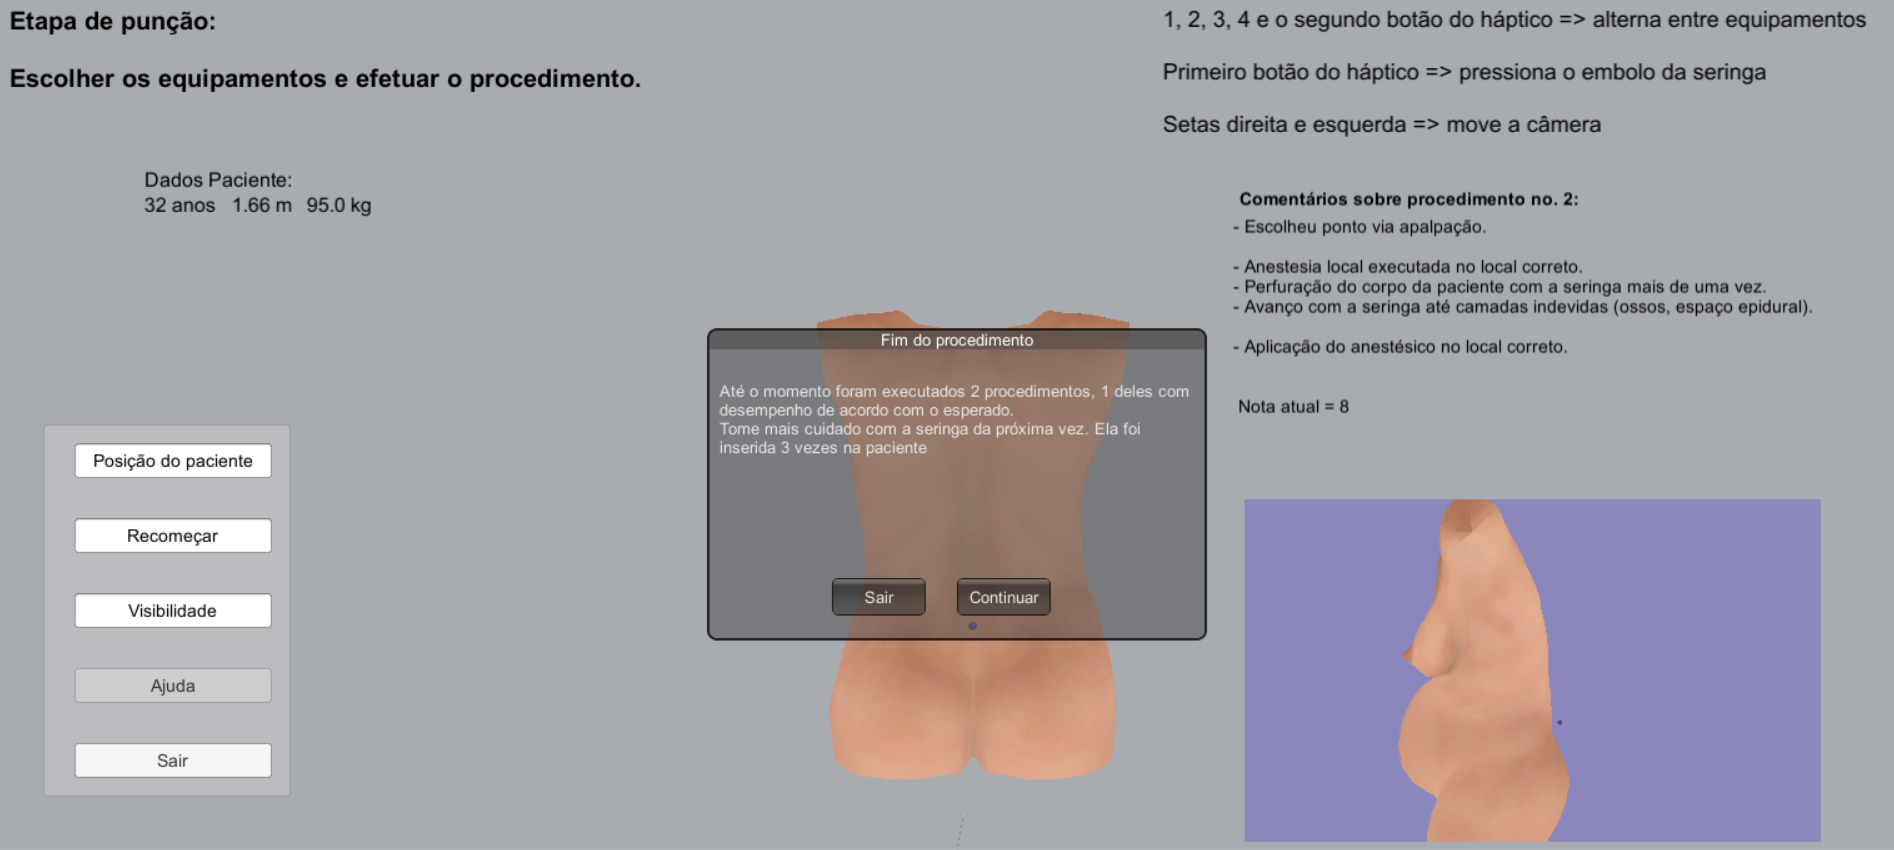
\includegraphics[width=\textwidth]{capitulos/figuras/sistema-exemplo-execucao-procedimento-2.png} 
    \caption{Exemplo de \textit{feedback} do ambiente após finalização de um segundo procedimento onde a seringa foi inserida mais de três vezes no corpo da paciente e partes indevidas foram tocadas.}
    \label{fig:sistemaExecucao2seringaCorreto}
\end{figure}

\begin{figure}[ht!]
    \centering
    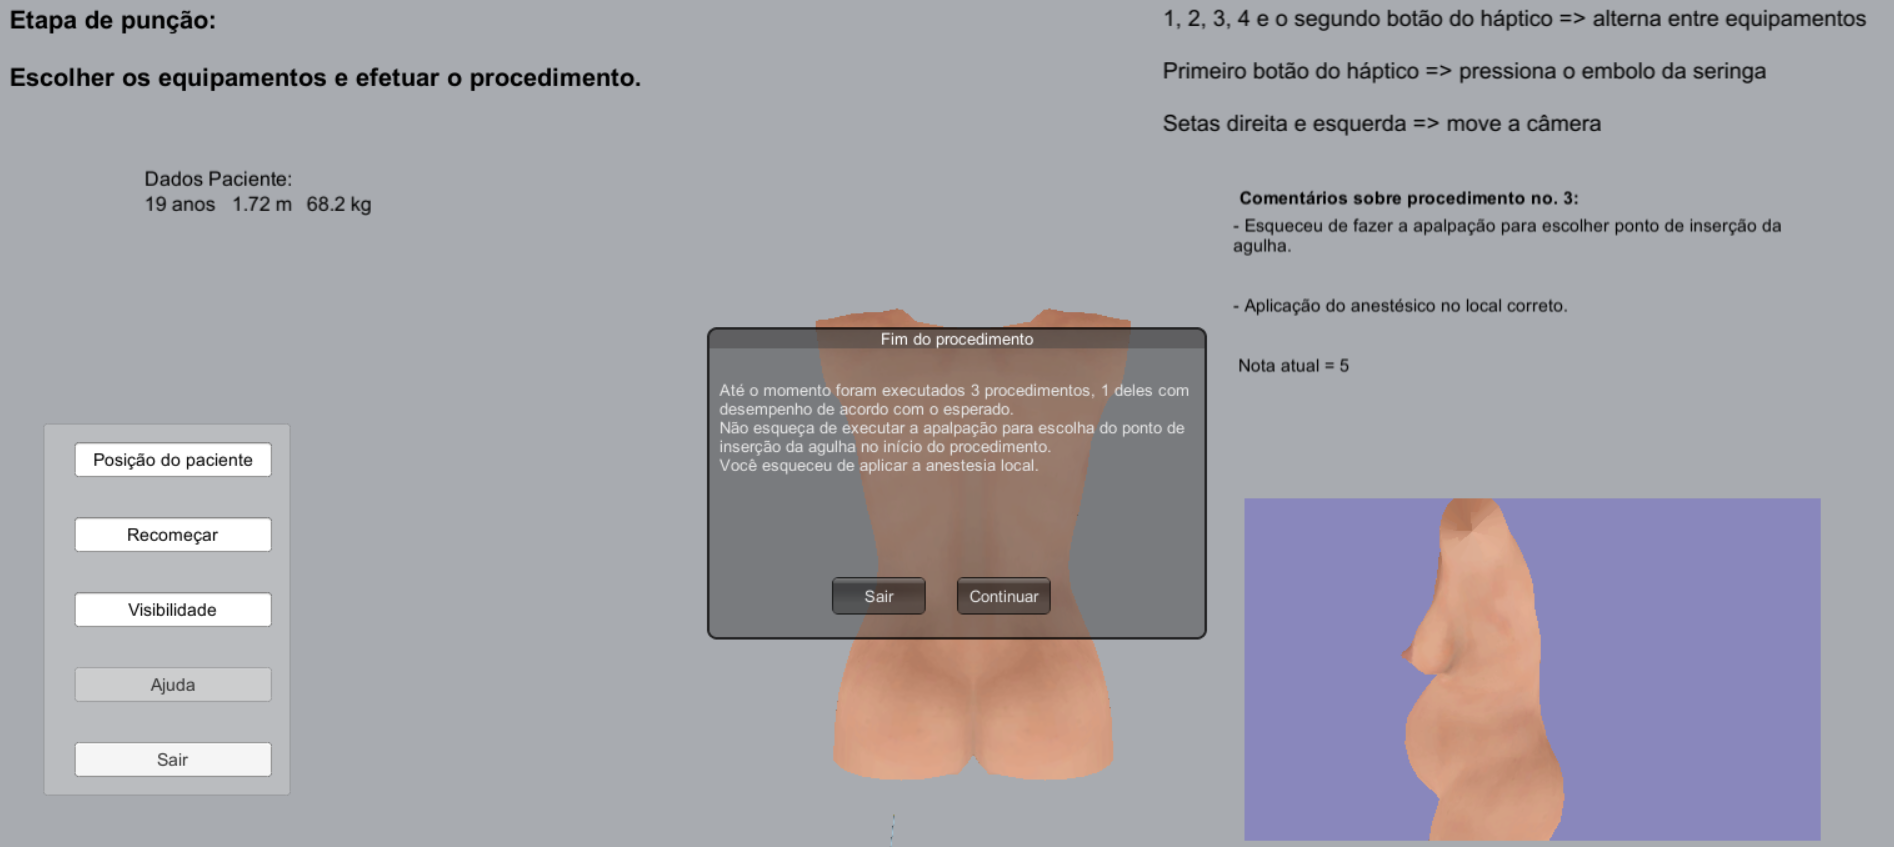
\includegraphics[width=\textwidth]{capitulos/figuras/sistema-exemplo-execucao-procedimento-3.png} 
    \caption{Exemplo de \textit{feedback} do ambiente após finalização de um terceiro procedimento, onde o usuário não fez a palpação para escolher o ponto de inserção da agulha e nem aplicou a anestesia local antes de inserção da agulha de raquianestesia.}
    \label{fig:sistemaExecucao3faltouApalpacaoAnestesiaLocalIncorreto}
\end{figure}

\begin{figure}[ht!]
    \centering
    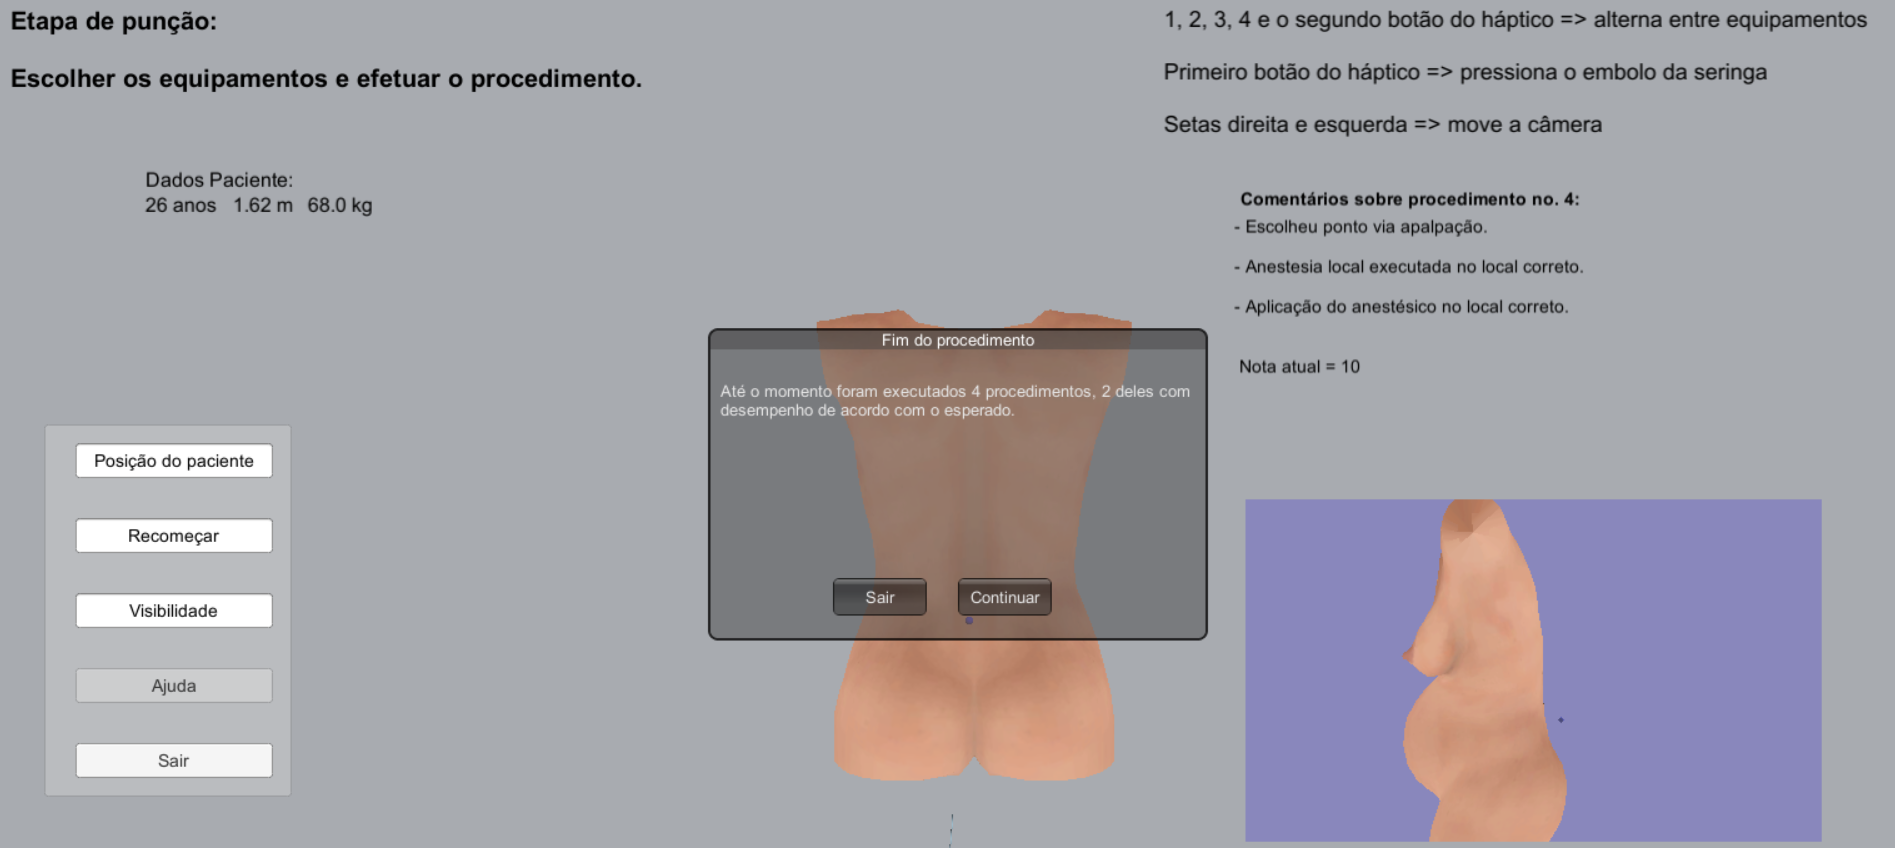
\includegraphics[width=\textwidth]{capitulos/figuras/sistema-exemplo-execucao-procedimento-4.png} 
    \caption{Tela do sistema após finalização de um quarto procedimento em que todo o procedimento foi executado de forma correta.}
    \label{fig:sistemaExecucao4correto}
\end{figure}

\begin{figure}[ht!]
    \centering
    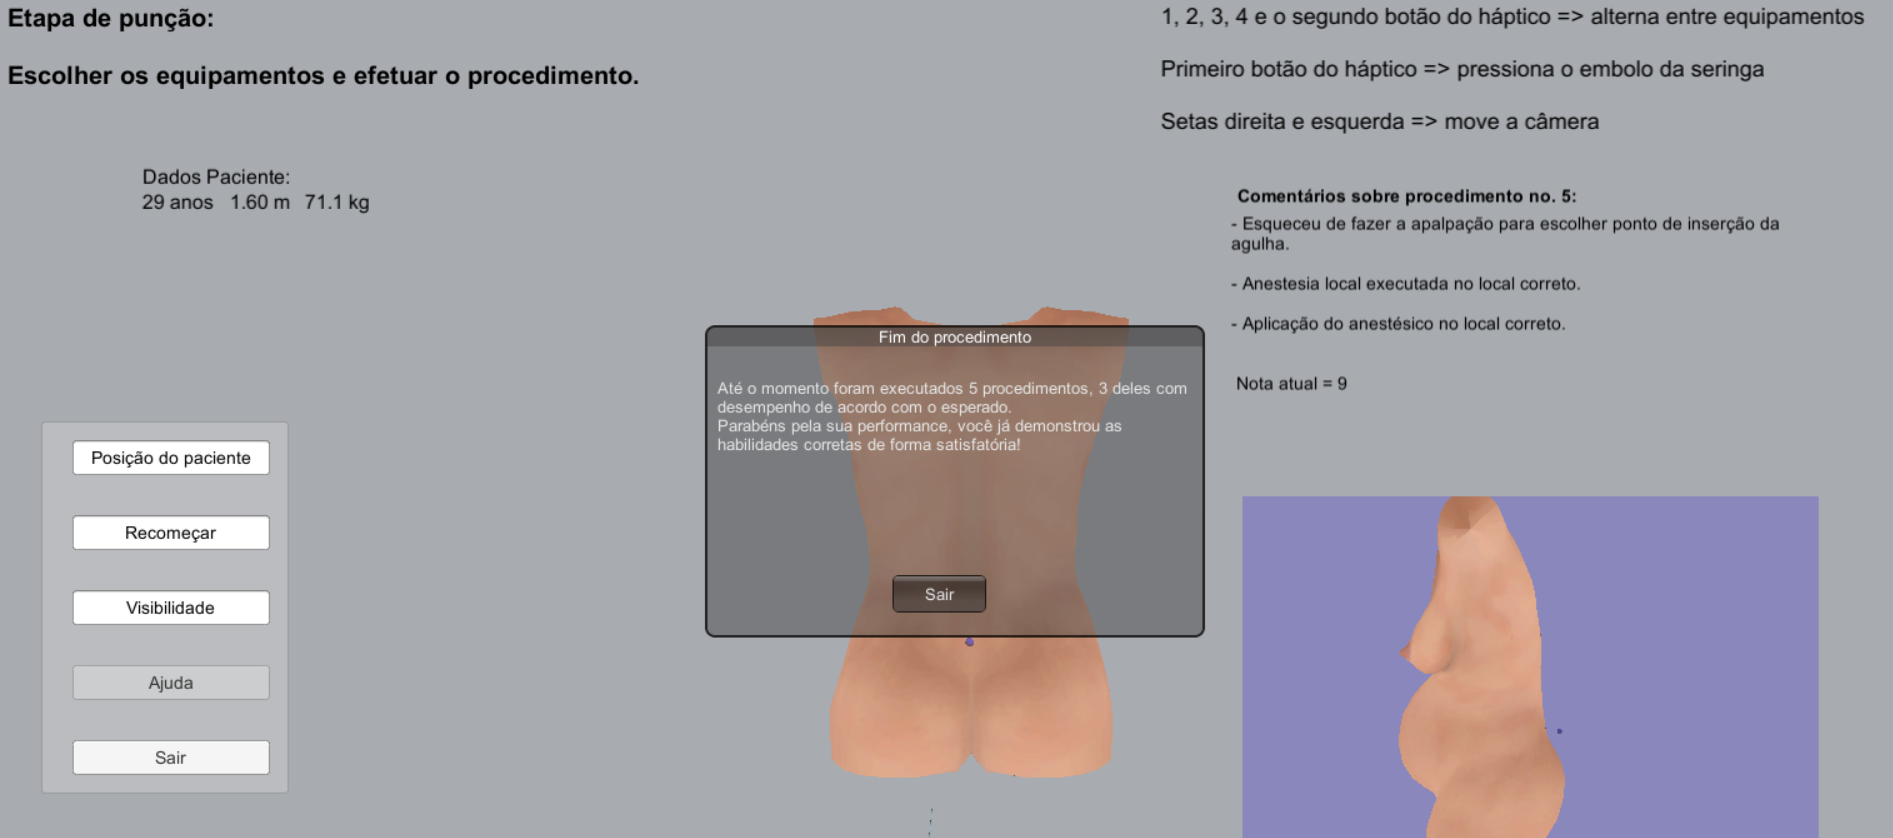
\includegraphics[width=\textwidth]{capitulos/figuras/sistema-exemplo-execucao-procedimento-5.png} 
    \caption{Exemplo de \textit{feedback} do ambiente após finalização de um quinto procedimento onde só não foi feita a palpação para determinação do ponto de inserção da agulha.}
    \label{fig:sistemaExecucao5semApalpacaoCorreto}
\end{figure}

As Figuras \ref{fig:sistemaExecucao1RaquiLocalIncorreto} e \ref{fig:sistemaExecucao3faltouApalpacaoAnestesiaLocalIncorreto} ilustram execuções de procedimentos onde as execuções foram abaixo da média (nota menores que seis) e, portanto, consideradas de desempenho não satisfatório. Na Figura \ref{fig:sistemaExecucao1RaquiLocalIncorreto}  nota um (1) foi obtida pois o usuário fez corretamente a palpação para determinação do ponto de inserção da agulha e fez uma correta aplicação da anestesia local, porém aplicou a raquianestesia no local indevido. Já na Figura \ref{fig:sistemaExecucao3faltouApalpacaoAnestesiaLocalIncorreto} o erro foi ter esquecido de fazer tanto a palpação pra escolha do ponto de inserção da agulha quanto a aplicação da anestesia local, mas foi aplicada corretamente a raquianestesia, o que fez receber cinco como nota final no procedimento. Os outros três procedimentos foram efetuados com resultados acima da média sendo um deles (Figura \ref{fig:sistemaExecucao4correto}) com a nota máxima (dez) por não ter cometido nenhum erro ou esquecimento. No procedimento representado pela Figura \ref{fig:sistemaExecucao5semApalpacaoCorreto} a nota final foi nove, pois, o único erro foi o de esquecimento da palpação para determinação do ponto de inserção da agulha. Na Figura \ref{fig:sistemaExecucao2seringaCorreto} os erros de execução no procedimento foram a perfuração do corpo da paciente mais de três vezes com a seringa e avanço desta para camadas indevidas o que fez com que a nota final para este caso fosse sete. 
Após os cinco procedimentos efetuados, uma vez que três deles tiveram notas acima da média e, a média da nota de todos os cinco procedimentos foi maior que seis (somatório das cinco notas foi de 32) o usuário foi parabenizado pela sua performance e não foi necessário continuar com os treinamentos. Esta sequência de telas ilustra um treinamento usando o simulador desde o seu início até o final. Um vídeo que ilustra toda a execução de um procedimento, assim como uma visão geral do ambiente de treinamento desenvolvido nesta tese pode ser visto no link\footnote{\url{https://youtu.be/g9RZRYId9ys}}. Para demonstrar as funcionalidades dos botões laterais, incluindo a transparência das camadas e em parte o \textit{feedback} dado durante o procedimento foi gravado um outro vídeo que pode ser visto no link\footnote{\url{https://youtu.be/gGpJKjkVYWU}}.

Foi inserida no sistema uma opção de execução que guia o usuário mais inexperiente nas etapas da raquianestesia que estão disponíveis no ambiente de treinamento desenvolvido. Essa opção foi denominada de tutorial. Ao ser ativada, através do botão de nome tutorial, na área inferior à esquerda da tela, a transparência do corpo da paciente é habilitada e textos explicativos da etapa atual de cada procedimento são exibidos na área superior à esquerda da tela, como pode ser visto nas Figuras \ref{fig:sistemaExecucaoTutorialApalpacao}, \ref{fig:sistemaExecucaoTutorialAnestesiaLocal}. Nos textos destas telas, na primeira linha, é identificado o elemento de interação que está atualmente selecionado no ambiente virtual. O elemento de interação que representa o dedo do médico está selecionado na Figura \ref{fig:sistemaExecucaoTutorialApalpacao}, este sempre está selecionado ao iniciar um novo procedimento. Os demais elementos de interação existentes são a seringa de anestesia local, a agulha de raquianestesia e a agulha de raquianestesia com a seringa conectada a ela. Ainda nesta imagem, no modo tutorial, é falado sobre a primeira escolha que deve ser feita que é a da posição da paciente e a subsequente palpação para identificação do ponto de inserção da agulha. 

\begin{figure}[ht!]
    \centering
    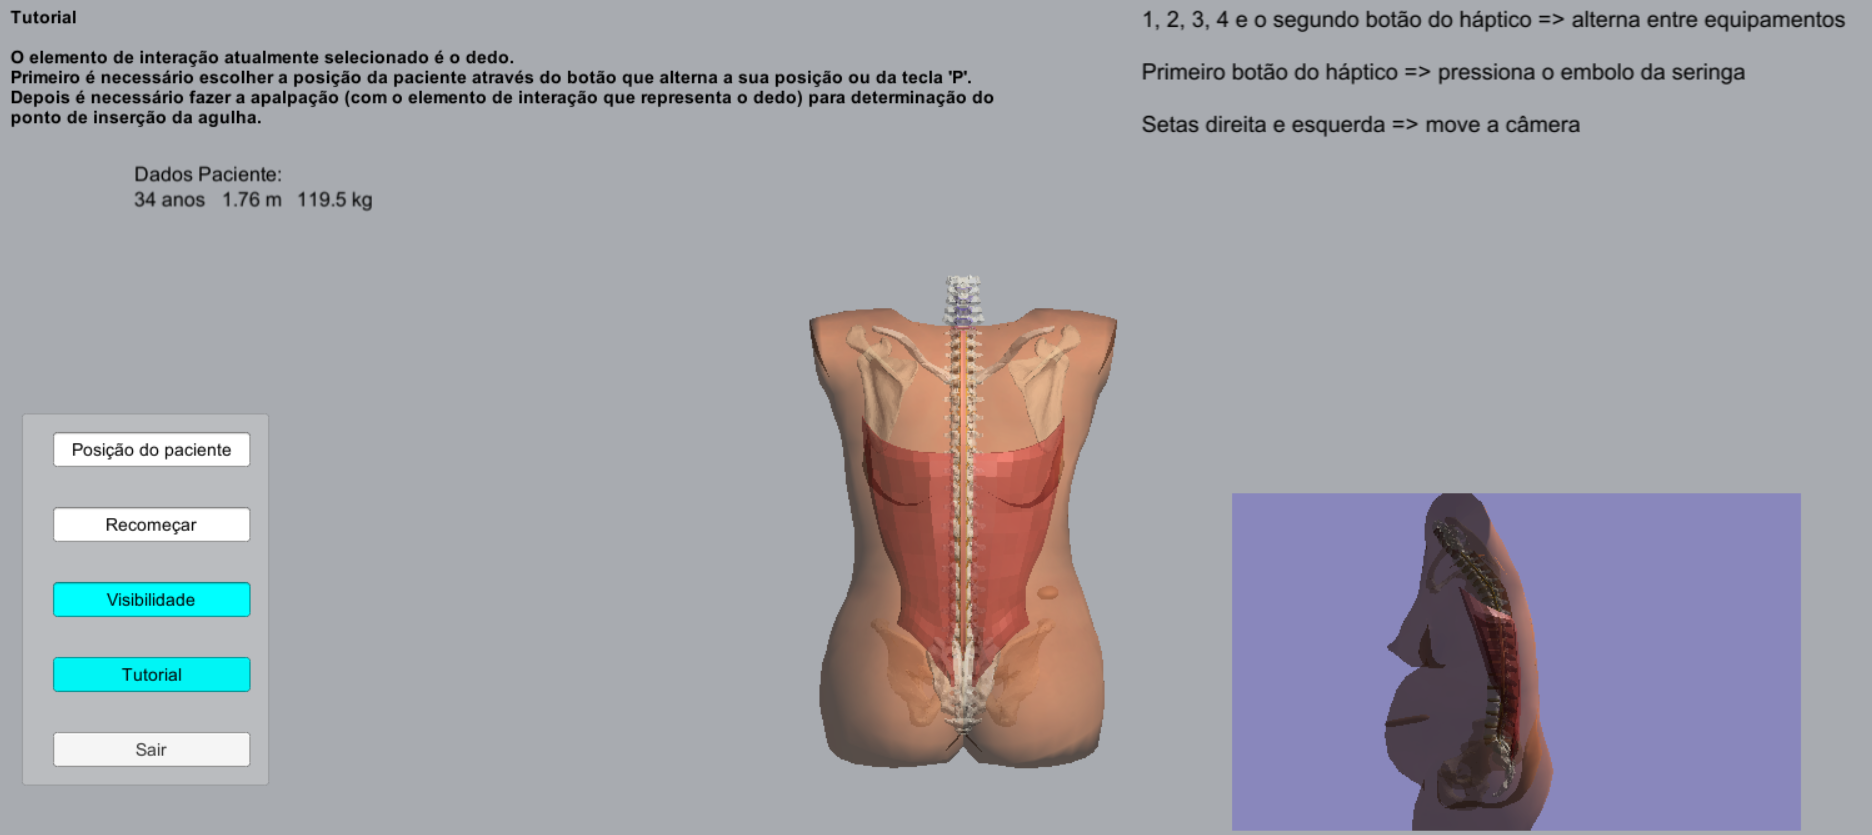
\includegraphics[width=\textwidth]{capitulos/figuras/sistemaExecucaoTutorialApalpacao.png} 
    \caption{Exemplo do \textit{feedback} do modo tutorial no ambiente no início do procedimento.}
    \label{fig:sistemaExecucaoTutorialApalpacao}
\end{figure}

\begin{figure}[ht!]
    \centering
    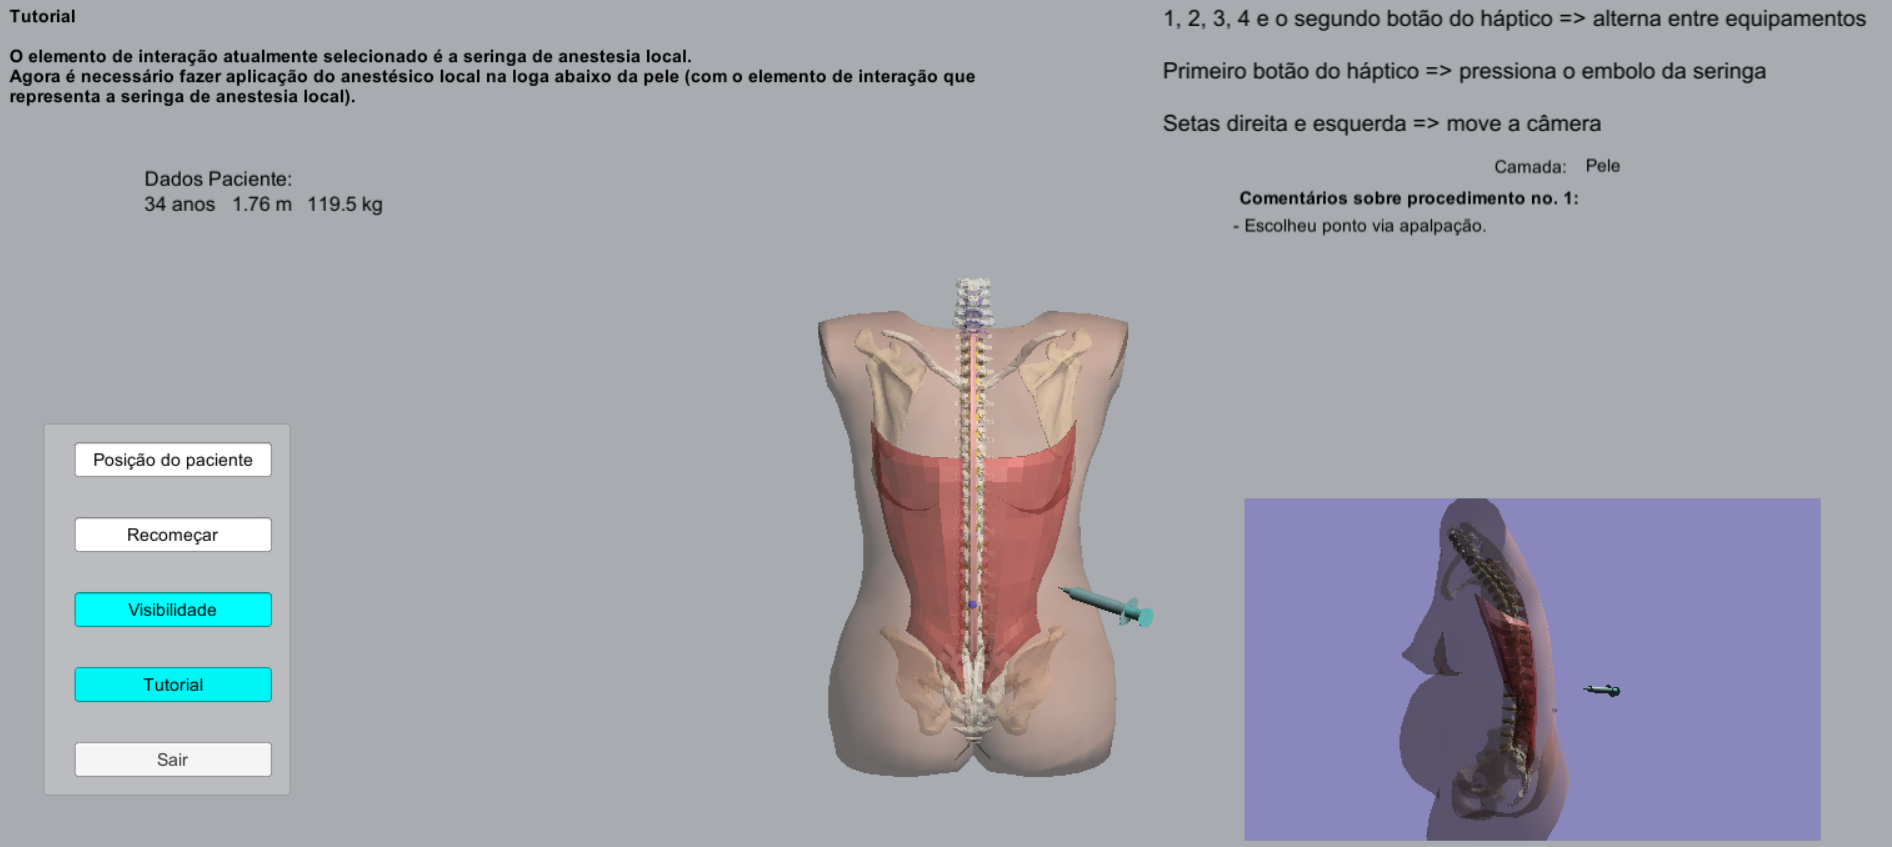
\includegraphics[width=\textwidth]{capitulos/figuras/sistemaExecucaoTutorialAnestesiaLocal.png} 
    \caption{Exemplo do \textit{feedback} do modo tutorial no ambiente após a escolha do ponto de inserção da agulha via palpação.}
    \label{fig:sistemaExecucaoTutorialAnestesiaLocal}
\end{figure}

A Figura \ref{fig:sistemaExecucaoTutorialAnestesiaLocal} ilustra o texto que é exibido após ter sido feita a escolha do ponto de inserção da agulha. É, portando, falado sobre qual equipamento deve ser usado para efetuar o próximo passo do procedimento que é a anestesia local. Uma vez feita a anestesia local (no modo tutorial), o usuário é então informado sobre qual é a etapa a ser feita para finalização do procedimento. O sistema também informa com que equipamento e em que camada a raquianestesia deve ser aplicada como pode ser visto na Figura \ref{fig:sistemaExecucaoTutorialRaqui}. Esta imagem ilustra que é possível remover a transparência das camadas (clicando no botão Visibilidade) e ainda continuar recebendo as ajudas do modo tutorial. Isto foi feito de forma ao sistema possibilitar níveis de ajuda distintos, dependendo das necessidades do usuário além de tornar o sistema mais autoexplicativo. 

\begin{figure}[ht!]
    \centering
    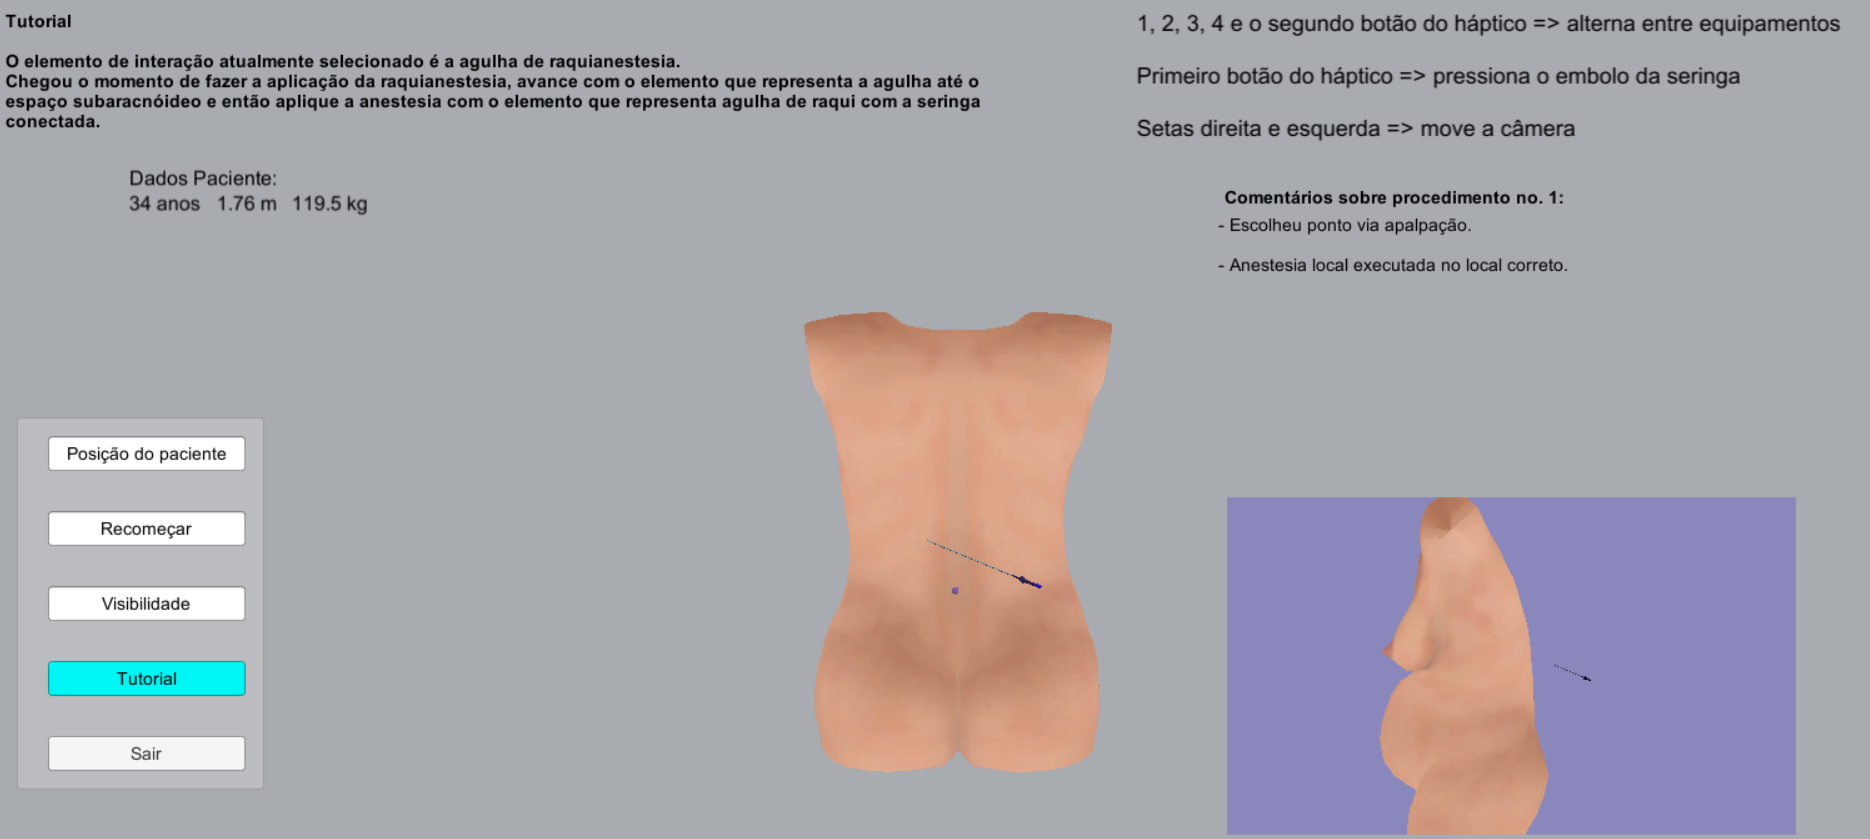
\includegraphics[width=\textwidth]{capitulos/figuras/sistemaExecucaoTutorialRaqui.png} 
    \caption{Tela do sistema no modo tutorial após a anestesia local ter sido efetuada.}
    \label{fig:sistemaExecucaoTutorialRaqui}
\end{figure}

Na Figura \ref{fig:sistemaExecucaoVisibilidadeCamadaAtual} é ressaltado na tela do sistema a parte da informação sobre o tecido (camada) do corpo que foi tocada por último pelo elemento de interação (agulha de raquianestesia para esta imagem). Esta informação é exibida sempre que a transparência das camadas está habilitada. Esta informação é útil no treinamento ao possibilitar o reconhecimento das sensações experimentadas ao tocar (e transpassar) cada camada pela agulha de raquianestesia. Isto serve tanto para o treinamento de novos anestesistas inexperientes quanto para a validação destas sensações por anestesistas experientes, que é um próximo passo natural na continuação do desenvolvimento deste ambiente de treinamento. Um outro momento em que a informação da camada sendo tocada é exibida nesta mesma posição é quando, mesmo sem a transparência ativada, a ponta da agulha está posicionada no espaço subaracnóideo. Isto foi feito para substituir a dica visual do procedimento real, pois neste, quando a agulha atinge este espaço há o escorrimento de líquor pela agulha.  

\begin{figure}[ht!]
    \centering
    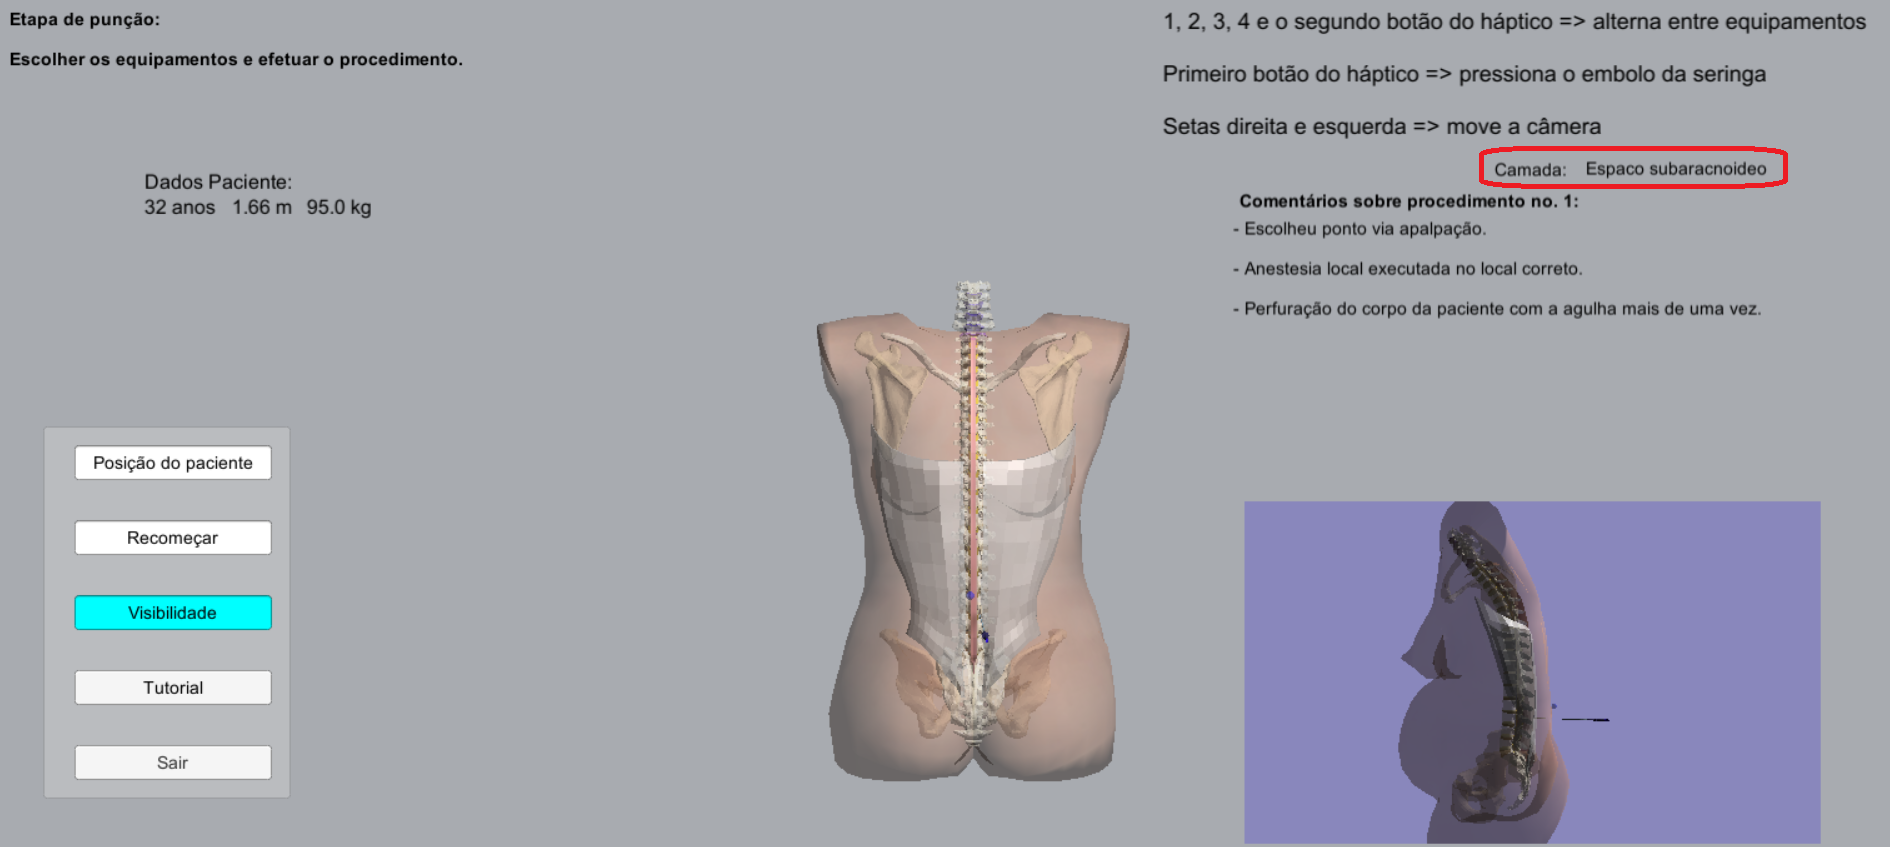
\includegraphics[width=\textwidth]{capitulos/figuras/sistemaExecucaoCamadaAtual.png} 
    \caption{Demonstração do ambiente funcionando com a  transparência das camadas ativada. A informação da camada atualmente tocada pela agulha está marcada em vermelho.}
    \label{fig:sistemaExecucaoVisibilidadeCamadaAtual}
\end{figure}